% Figure 1: packed alignment positions divided into tiles. Shared by the
% standalone preview and the paper; the enclosing document defines \figurefont.
\definecolor{ink}{HTML}{252525}
\definecolor{utteranceone}{HTML}{DBE9F3}
\definecolor{utterancetwo}{HTML}{F2E5CC}

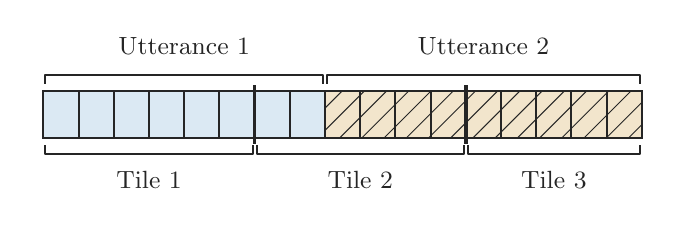
\begin{tikzpicture}[
  x=1mm, y=1mm, draw=ink, text=ink,
  font=\small\figurefont,
  every node/.style={inner sep=0pt, outer sep=0pt, anchor=base,
                    yshift=-2.484375bp, execute at begin node=\vphantom{g}},
  bracket/.style={line width=.65bp, line cap=rect, line join=round}]
  \path[use as bounding box] (0,0) rectangle (80,22);
  \begin{scope}[overlay]
    \pgfmathsetmacro{\pitch}{76/17}
    \pgfmathsetmacro{\boundary}{2+8*\pitch}

    % Seventeen valid rows, grouped by utterance and divided into three tiles.
    \foreach \i in {0,...,16} {
      \ifnum\i<8
        \fill[utteranceone] ({2+\i*\pitch},8) rectangle ++(\pitch,6);
      \else
        \fill[utterancetwo] ({2+\i*\pitch},8) rectangle ++(\pitch,6);
      \fi
    }
    \begin{scope}
      \clip (\boundary,8) rectangle (78,14);
      \foreach \i in {0,...,40} {
        \draw[line width=.35bp] ([xshift={8*\i bp}]-22,0) -- ++(80,80);
      }
    \end{scope}
    \foreach \i in {0,...,16}
      \draw[line width=.7bp] ({2+\i*\pitch},8) rectangle ++(\pitch,6);

    \foreach \a/\b/\name in {2/\boundary/1,\boundary/78/2} {
      \draw[bracket] ({\a+.25},15) -- ({\a+.25},16)
        -- ({\b-.25},16) -- ({\b-.25},15);
      \node at ({(\a+\b)/2},19.5) {Utterance \name};
    }
    \foreach \i in {6,12}
      \draw[line width=1.25bp, line cap=rect]
        ({2+\i*\pitch},7.5) -- ({2+\i*\pitch},14.5);
    \foreach \a/\b/\name in {0/6/1,6/12/2,12/17/3} {
      \draw[bracket] ({2+\a*\pitch+.25},7) -- ({2+\a*\pitch+.25},6)
        -- ({2+\b*\pitch-.25},6) -- ({2+\b*\pitch-.25},7);
      \node at ({2+(\a+\b)*\pitch/2},2.5) {Tile \name};
    }
  \end{scope}
\end{tikzpicture}
